\section{Class diagram}

\fxnote{Hele det har afsnit burde blive auto-generated af doxygen (Så comments står inde i koden istedet) - JH}

%\fxnote{Der mangler en navngivnings standard, f.eks. hvis jeg gør brug af init() metoden, hvordan ved jeg hvor jeg skal find implementationen? Evt. følg psoc's egen <ModulNavn>\_<Function>(), så det ville blive ControllerClass\_Init() - JH}

\fxnote{De fleste klasser har heller ikke sigende navne - JH}

%\fxnote{Skift designet på samtlige diagrammer! Ville være umuligt at læse i sort-hvid print, er allerede svært nu (Brug den klassiske hvid/lyse-blå i visio) - JH}
\begin{figure}[H]
	\centering
	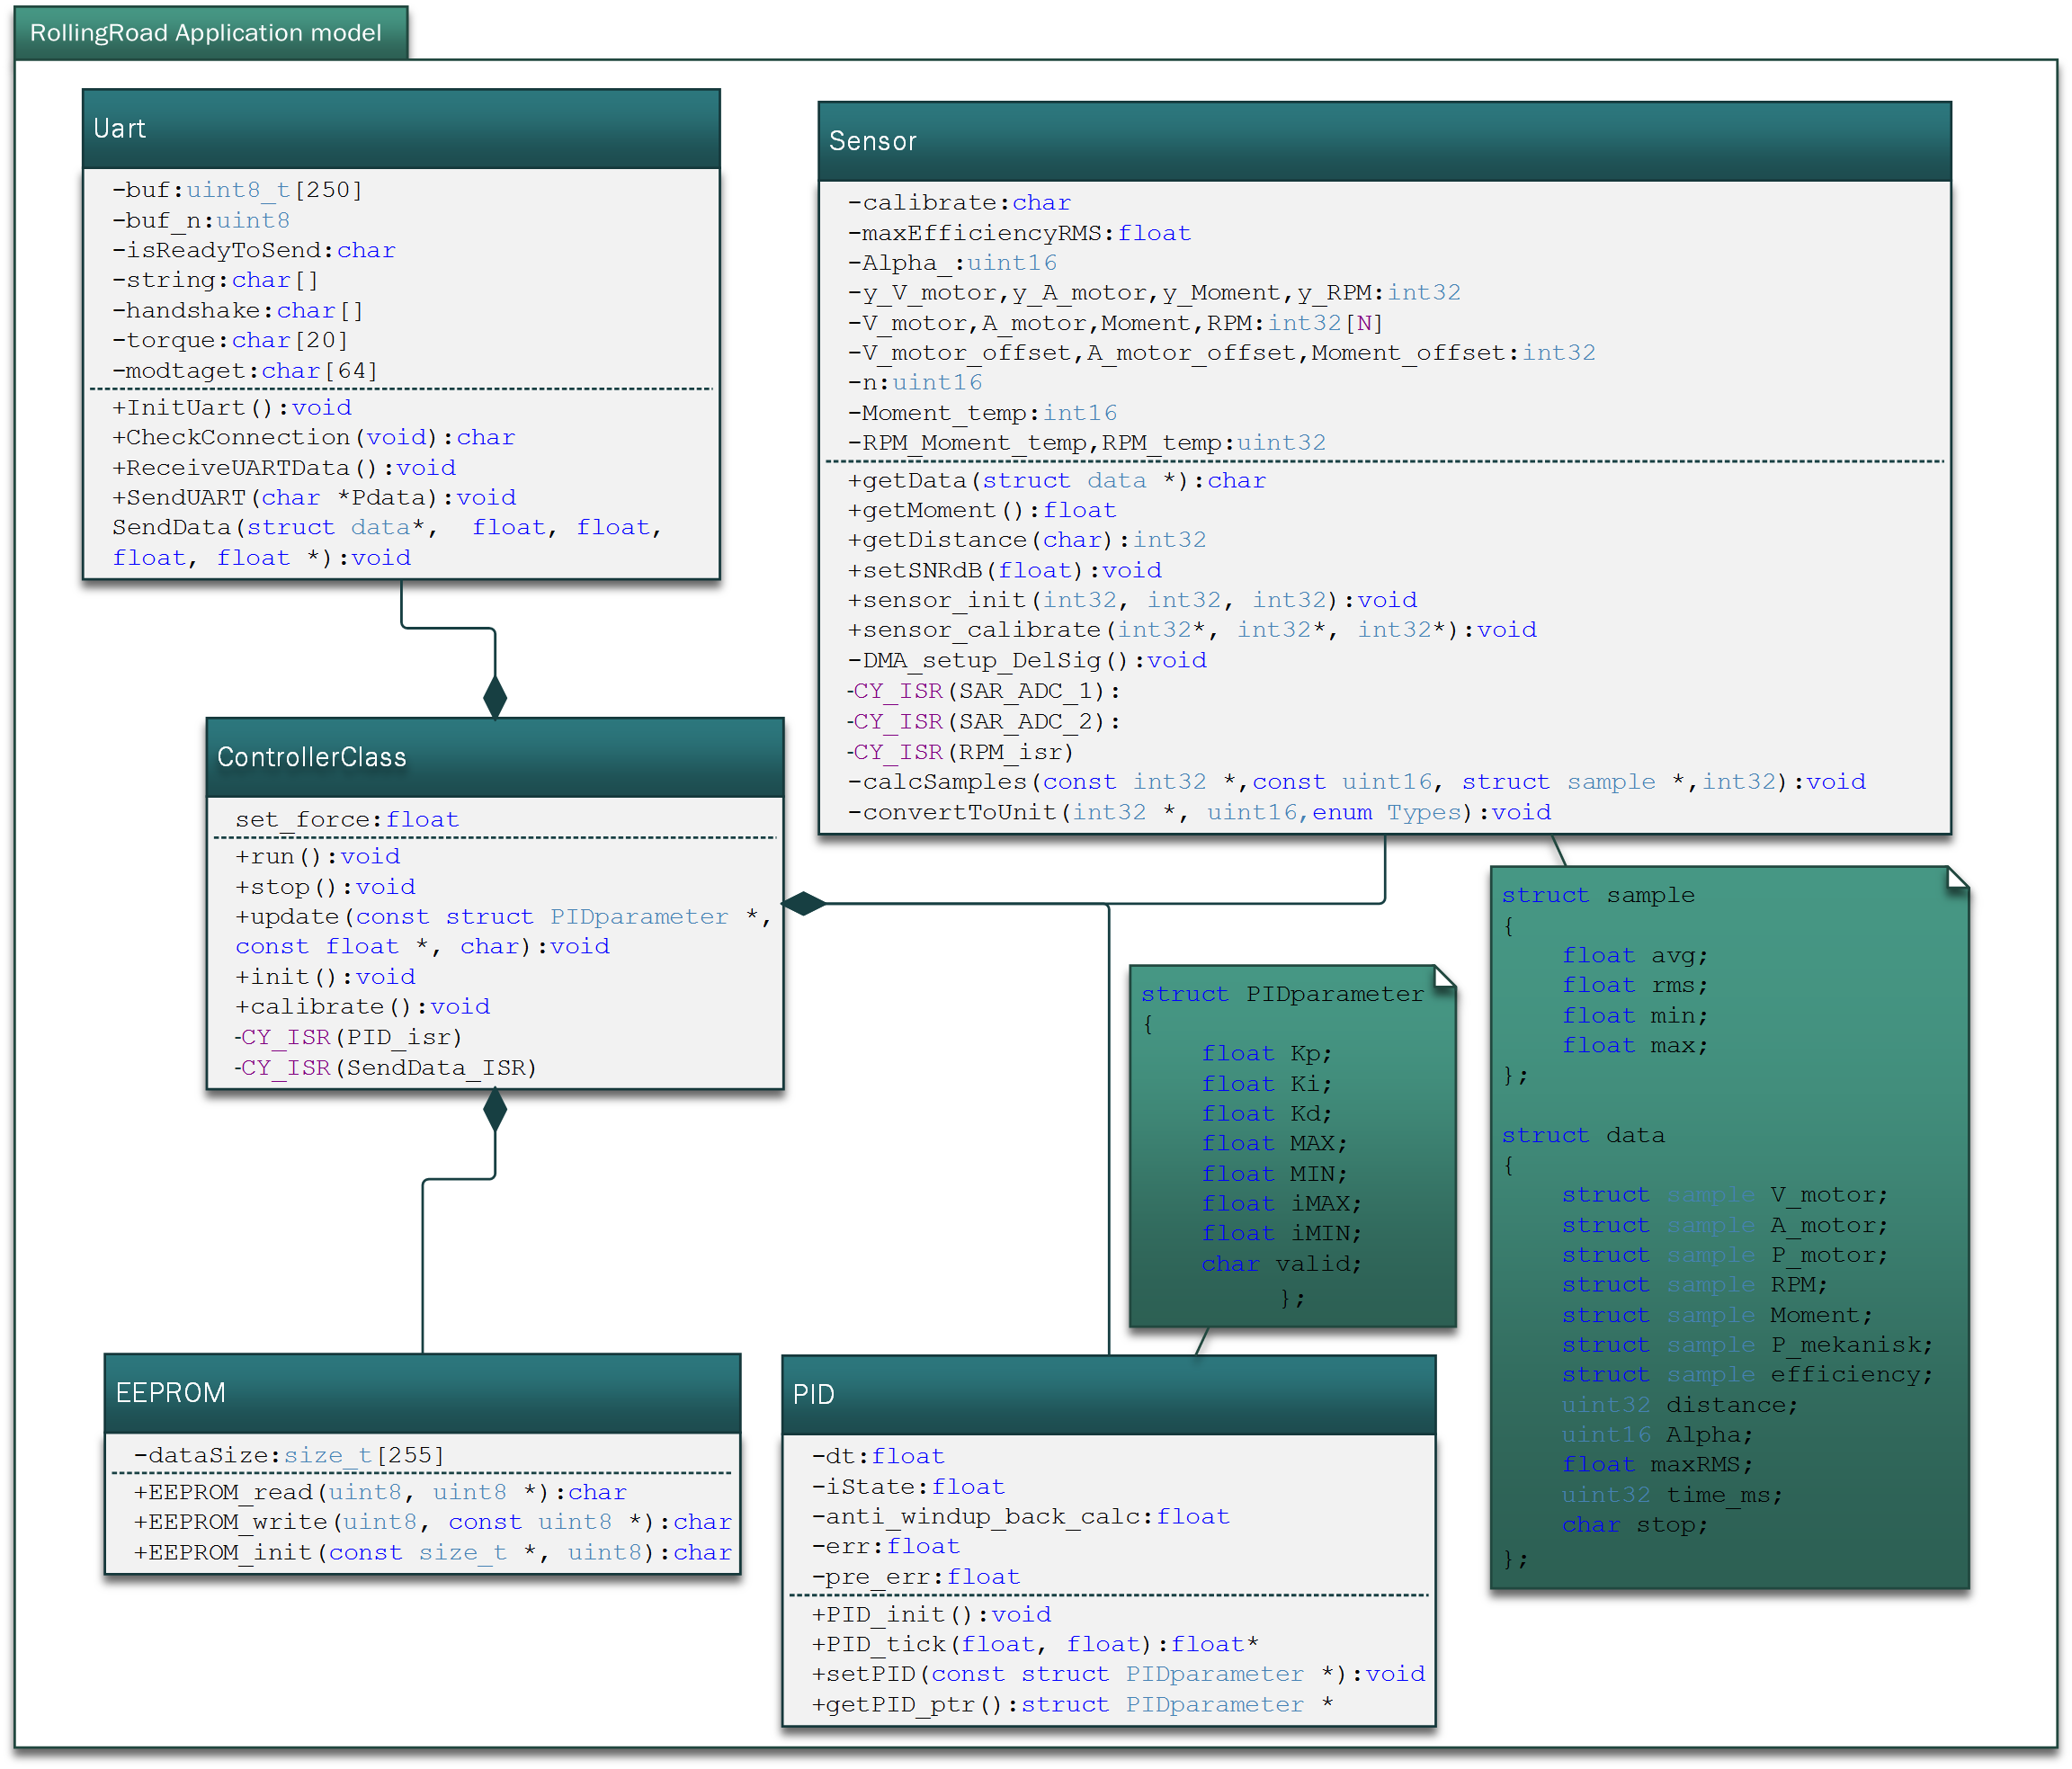
\includegraphics [width=6in]{Software/Pictures/klassediagram.png}
	\caption{Class diagram of Rolling Road PSoC}
	\label{fig:Class_diagram_RR_PSoC}
\end{figure}

The Class diagram of Rolling Road \vref{fig:Class_diagram_RR_PSoC}. 5 class where all class are connect to the ControllerClass which control the flow in sequencing of the program.\\
Uart class: is the class that communicate with the control panel through UART. It both send new data and receive settings and commands from the control panel. \\
EEPROM class: make it possible to save data too the EEPROM on the PSoC. It can be PID parameters and offset values to all sensors.\\
PID class: job is to regulate the load system, so the wanted Torque is reached. \\
Sensor class: are measuring the efficiency of the test object.

\section{Class description}

\subsection{ControllerClass}

\begin{figure}[H]
	\centering
	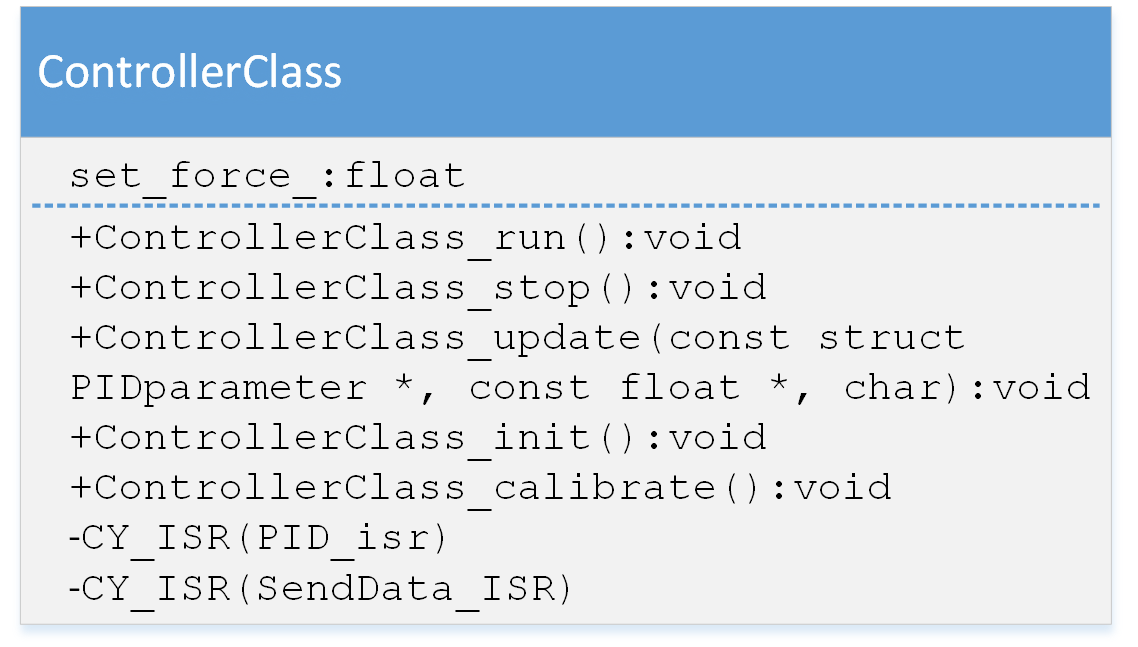
\includegraphics [width=3in]{Software/Pictures/klassediagram_ControllerClass.png}
	\caption{ControllerClass of Rolling Road PSoC}
	\label{fig:Class_diagram_ControllerClass_RR_PSoC}
\end{figure}

\begin{table}[H]
	\centering
	\begin{tabular}{|p{5 cm}|p{10 cm}|}
		\hline
		\textbf{methods} & \textbf{Description} \\ \hline
		
		ControllerClass\_run
		& Is the method what check if there is new data ready from the main PC or if where is a new sample ready to send to the main PC. Data from the PC can be PID values, wanted force value or commands to ex. calibrate all sensors. 
		\\ & It is also here that the main thread have to work, and should be placed in a while(1) loop. \\ 
		\hline
		
		ControllerClass\_stop
		& This method are used to tell Rolling Road that no more information is wanted, and it don't have to regulate the load system. 
		\\ \hline
		
		ControllerClass\_update
		& Update method are called then new data for Rolling Road is received. This method is used by the UART class.
		\\ & \textbf{Parameter list}
		\\ & \begin{itemize}
			\item {\large const struct PIDparameter *}
			\subitem \textit{If this is not a null pointer, it is new PID values, an will be updated.}
			\item {\large const float *}
			\subitem \textit{If this is not a null pointer, it is a new wanted force an will update the old value.}
			\item {\large char}
			\subitem \textit{If not 0. It will reset the distance counter.}
		\end{itemize}
		\\ \hline
		
		ControllerClass\_init
		& this method is used to initializing Rolling Road, and should be run in the start of the main function.  
		\\ \hline
		
		ControllerClass\_calibrate
		& This method are used from the UART class so the main PC can signal to Rolling Road. That it shall perform a calibration of all sensor.
		\\ \hline
	\end{tabular}
	\caption{Class description ControllerClass}
	\label{table:Class_description_ControllerClass_RR_PSoC}
\end{table}

\subsection{EEPROM}

\begin{figure}[H]
	\centering
	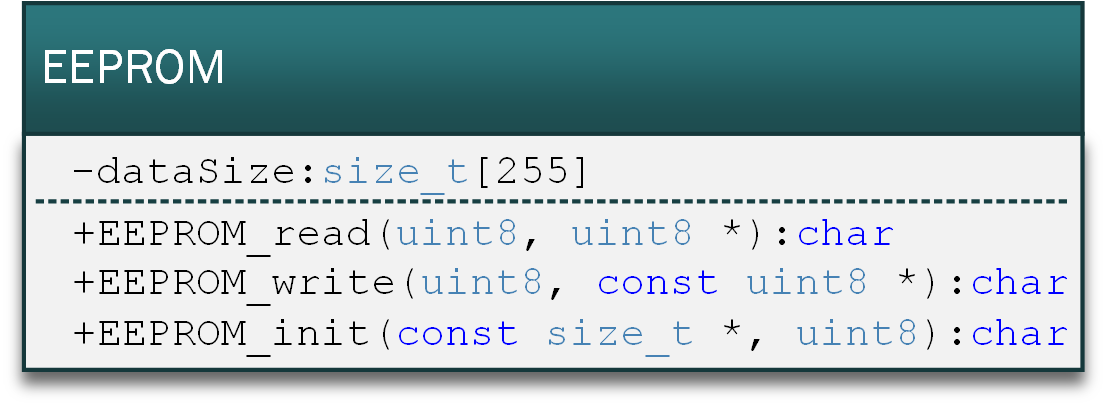
\includegraphics [width=3in]{Software/Pictures/klassediagram_EEPROM.png}
	\caption{EEPROM class of Rolling Road PSoC}
	\label{fig:Class_diagram_EEPROM_RR_PSoC}
\end{figure}


\begin{table}[H]
	\centering
	\begin{tabular}{|p{5 cm}|p{10 cm}|}
		\hline
		\textbf{methods} & \textbf{Description} \\ \hline
		
		EEPROM\_read
		& This method are used to read saved data from the EEPROM on the PSoC.
		\\ & \textbf{Return parameter}
		\\ & If the reading has succeeded it will return 1. If it fails to read from the EEPROM it return 0. Note it will also fail if there is no saved data.
		\\ & \textbf{Parameter list}
		\\ & \begin{itemize}
			\item {\large uint8}
			\subitem \textit{this parameter is used to choose the data you want to read, It just the ID of the content that has been saved.}
			\item {\large uint8*}
			\subitem \textit{A pointer to a buffer there the data will be saved to.}
		\end{itemize}
		\\ \hline
		
		EEPROM\_write
		& This method make it possible to save data to the EEPROM.
		\\ & \textbf{Return parameter}
		\\ & if it return 1, it has successfully write the data to the EEPROM. If it return -1 it has failed.
		\\ & \textbf{Parameter list}
		\\ & \begin{itemize}
			\item {\large uint8}
			\subitem \textit{this parameter is used to choose the data you want to save, It just the ID of the content you want to save.}
			\item {\large uint8*}
			\subitem \textit{A pointer to the data you want to saved. Note It will be a good idea to save it to the same data type, as you have defined in the initializing}
		\end{itemize}
		\\ \hline
		
		EEPROM\_init
		& It will initializing the class.
		\\ & \textbf{Return parameter}
		\\ & If it don't return 1, something is wrong and where is probably not enough memory in the EEPROM. If this method don't return 1 don't use the other methods!   
		\\ & \textbf{Parameter list}
		\\ & \begin{itemize}
			\item {\large const size\_t *}
			\subitem \textit{this parameter is used to send a array of sizes of data that will be saved on the EEPROM. The index of the arrays elements is also their IDs.}
			\item {\large uint8}
			\subitem \textit{This parameter is used to tell, have many elements there are in the array.}
		\end{itemize}
		\\ \hline

	\end{tabular}
	\caption{Class description EEPROM}
	\label{table:Class_description_EEPROM_RR_PSoC}
\end{table}

\subsection{PID}

\begin{figure}[H]
	\centering
	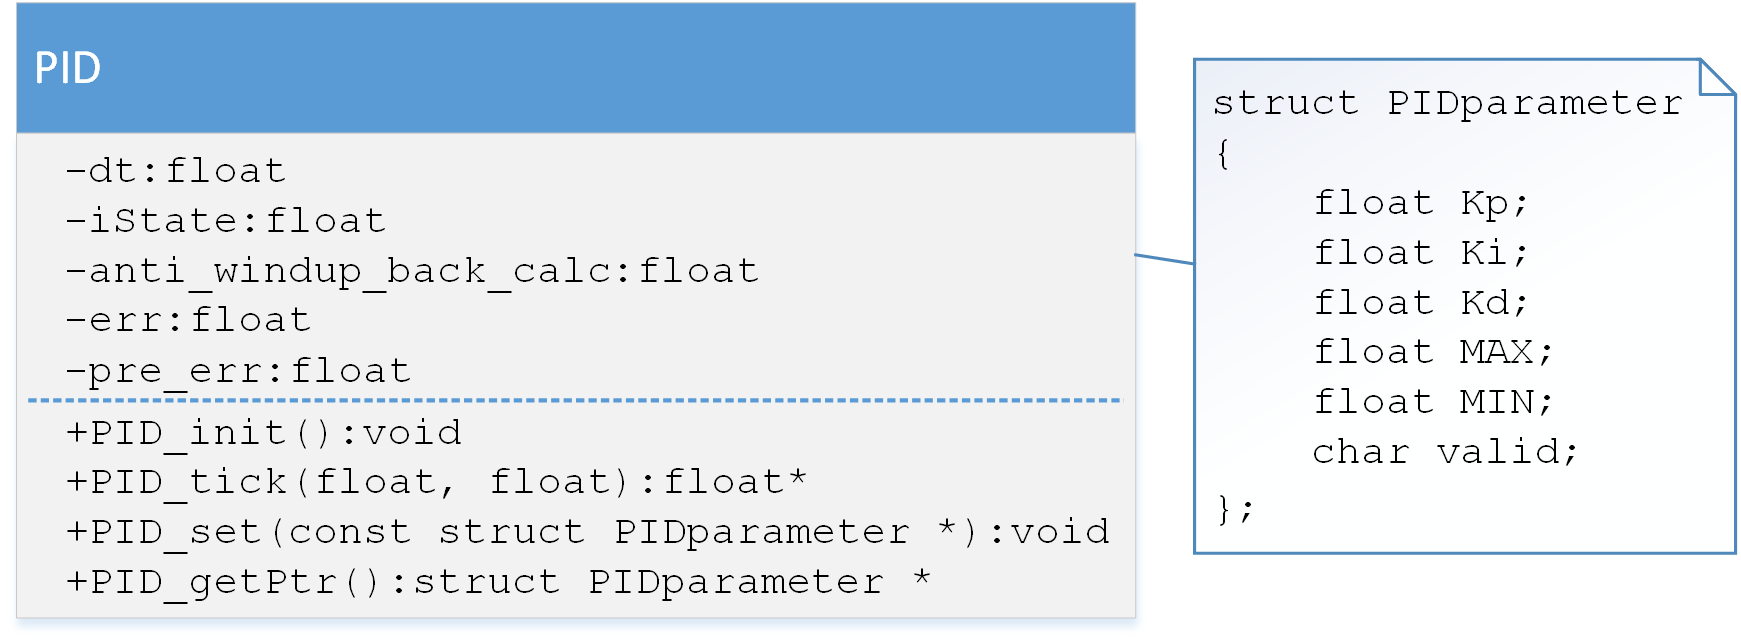
\includegraphics [width=3in]{Software/Pictures/klassediagram_PID.png}
	\caption{PID class of Rolling Road PSoC}
	\label{fig:Class_diagram_PID_RR_PSoC}
\end{figure}


\begin{table}[H]
	\centering
	\begin{tabular}{|p{5 cm}|p{10 cm}|}
		\hline
		\textbf{methods} & \textbf{Description} \\ \hline
		
		PID\_init
		& Initializing the class. 
		\\ \hline
		
		PID\_tick
		& This method should be executed periodic with constant time delay. 
		\\ & \textbf{Return parameter}
		\\ & The return parameter is only used to debug.
		\\ & \textbf{Parameter list}
		\\ & \begin{itemize}
			\item {\large float}
			\subitem \textit{Is the sensor/plant value}
			\item {\large float}
			\subitem \textit{Is the input value}
		\end{itemize}
		\\ \hline
		
		PID\_set
		& This method can change the PID values.
		\\ & \textbf{Parameter list}
		\\ & \begin{itemize}
			\item {\large const struct PIDparameter *}
			\subitem \textit{Change PID regulator parameter to a new sets of PID parameters}
		\end{itemize} 
		\\ \hline
		
		PID\_getPtr
		& return a pointer to its PID parameter.
		\\ & \textbf{Return parameter (struct PIDparameter *)}
		\\ & Return a pointer to the PID parameter. 
		\\ \hline
		
	\end{tabular}
	\caption{Class description PID}
	\label{table:Class_description_PID_RR_PSoC}
\end{table}

\subsection{Sensor} 

\begin{figure}[H]
	\centering
	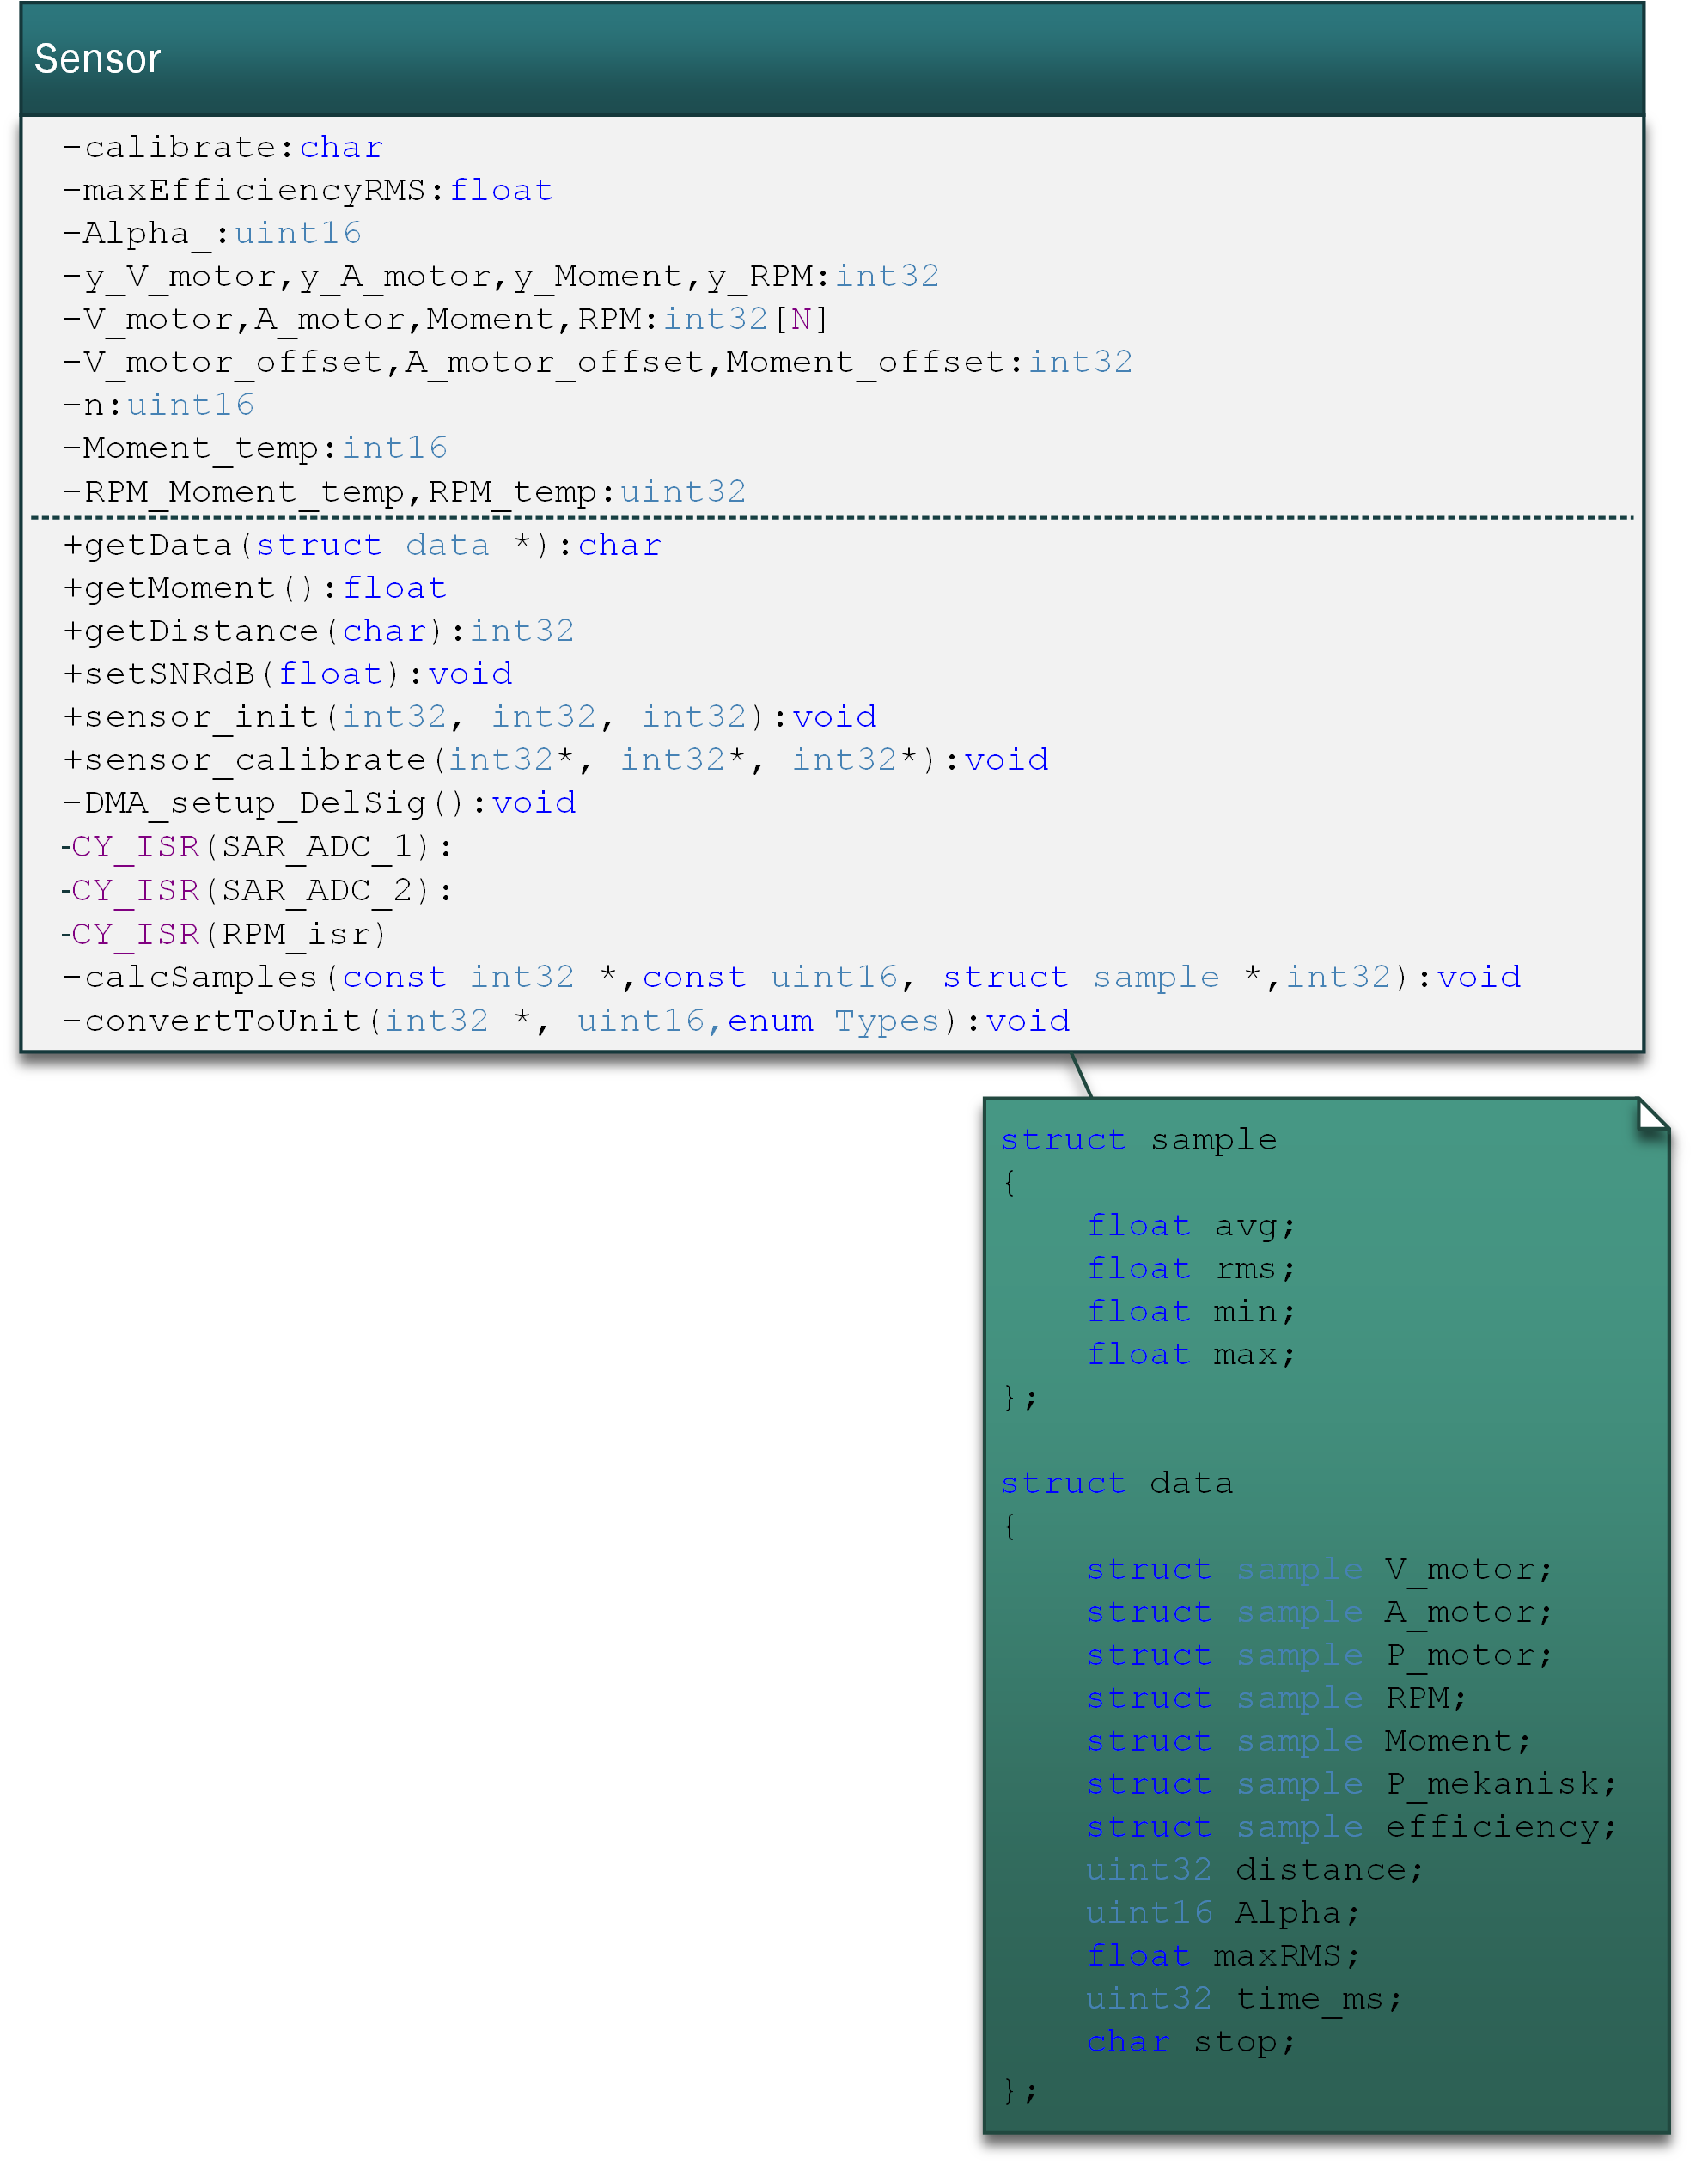
\includegraphics [width=5in]{Software/Pictures/klassediagram_sensor.png}
	\caption{Sensor class of Rolling Road PSoC}
	\label{fig:Class_diagram_Sensor_RR_PSoC}
\end{figure}


\begin{table}[H]
	\centering
	\begin{tabular}{|p{5 cm}|p{10 cm}|}
		\hline
		\textbf{methods} & \textbf{Description} \\ \hline
		
		Sensor\_getData
		& It will return a data sample.
		\\ & \textbf{Return parameter (void)}
		\\ & \textbf{Parameter list}
		\\ & \begin{itemize}
			\item {\large struct data *}
			\subitem \textit{A pointer to where the data will be saved.}
		\end{itemize}
		\\ \hline
		
		Sensor\_getTorque\fxnote{Skal have fixet - hilsten mig selv}
		& Are used to get the Torque without calculate all others values. In this project it is used by the PID class, to get the Torque value with less latency.
		\\ & \textbf{Return parameter (float)}
		\\ & It return the Torque value in $ N*m $ 
		\\ \hline
		
		Sensor\_getDistance
		& Gets the distance, Rolling Road has rolled. 
		\\ & \textbf{Return parameter (int32)}
		\\ & It return the distance in $ m $
		\\ & \textbf{Parameter list}
		\\ & \begin{itemize}
			\item {\large char}
			\subitem \textit{If 1 it will reset the counter, if 0 it will just return the distance.}
		\end{itemize}
		\\ \hline
			
			Sensor\_init
			& Initializing all sensor and DMA setup. It will also set offset value.   
			\\ & \textbf{Parameter list}
			\\ & \begin{itemize}
				\item {\large int32}
				\subitem \textit{Offset value to the Voltage sensor.}
				\item {\large int32}
				\subitem \textit{Offset value to the Current sensor.}
				\item {\large int32}
				\subitem \textit{Offset value to the Torque sensor.}
			\end{itemize}
			\\ \hline
			
			Sensor\_calibrate
			& Make a new calibration for Voltage-, Current and Torque sensor.    
			\\ & \textbf{Parameter list}
			\\ & \begin{itemize}
				\item {\large int32*}
				\subitem \textit{Return the offset value for the Voltage sensor.}
				\item {\large int32}
				\subitem \textit{Return the offset value for the Current sensor.}
				\item {\large int32}
				\subitem \textit{Return the offset value for the Torque sensor.}
			\end{itemize}
			\\ \hline
			
		\end{tabular}
		\caption{Class description Sensor}
		\label{table:Class_description_Sensor_RR_PSoC}
		
\end{table}




